\documentclass[review]{elsarticle}
%-----------------------------------------------------

\usepackage{amsmath}
\usepackage{graphicx}

\graphicspath{{./figs/}}

\newcommand{\ihat}{\boldsymbol{\hat{\textbf{\i}}}}
\newcommand{\jhat}{\boldsymbol{\hat{\textbf{\j}}}}
\newcommand{\roughly}{{\raise.17ex\hbox{$\scriptstyle\sim$}}}
\newcommand{\dmax}{d_\text{max}}
\newcommand{\dmin}{d_\text{min}}

%-----------------------------------------------------

\makeatletter
\renewcommand{\fnum@figure}{Figure 6}
\makeatother

\thispagestyle{empty}

\begin{document}
\allowdisplaybreaks

\begin{figure}[ht]
\centering
%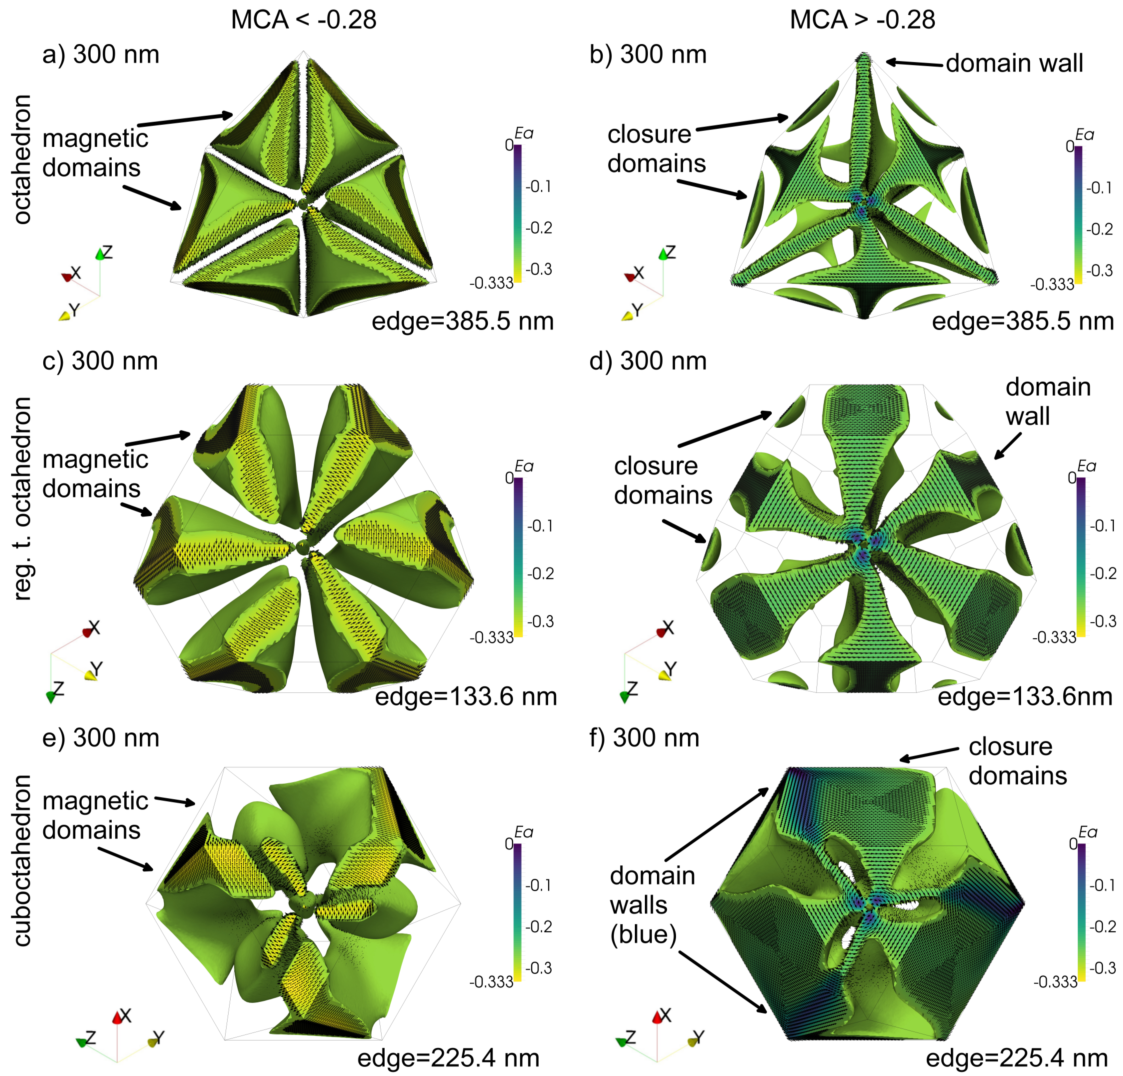
\includegraphics[width=\textwidth]{Figure_06_HR.pdf}
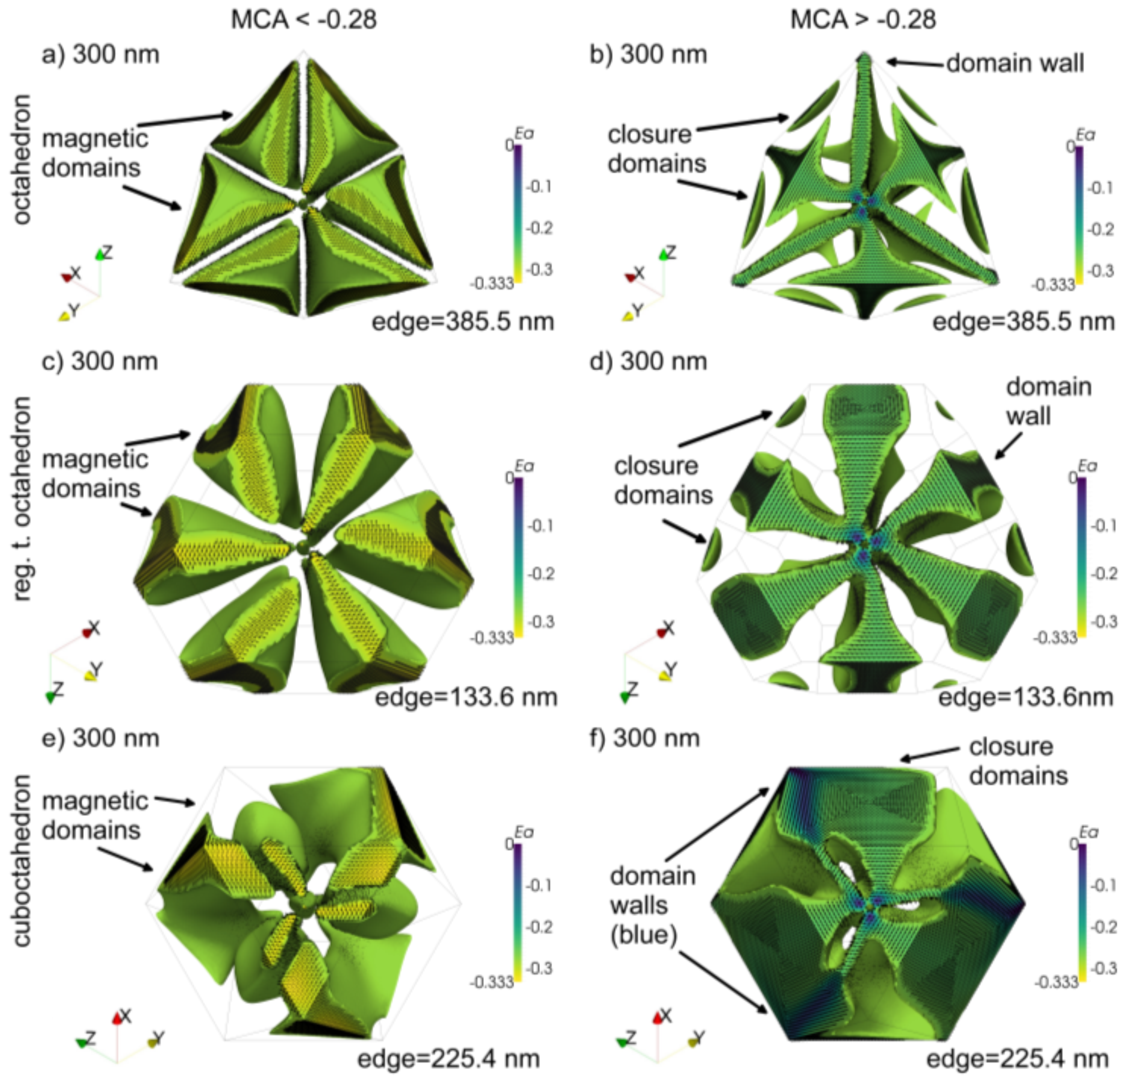
\includegraphics[width=\textwidth]{Figure_06.pdf}
\caption{MD formation by easy aligned vortices. From the solutions obtained by growing the 120$\,\text{nm}$ EAVs up to 300$\,\text{nm}$, the mesh nodes with MCA energy $<$-0.28 (normalised by $|K_1|$) are shown in the left column (a, c, e). These are regions which deviate from an easy axis alignment by less than $\roughly$15$^{\circ}$. The complement is shown in the right column: the regions with moderate to high ($>$-0.28) MCA energy (b, d, f). In the octahedron, there form six large magnetic domains filling up most of the volume (a) and narrow, flat regions acting as domain walls and small wedge-like regions formed along the edges interpreted as closure domains (b). The regular truncated octahedron EAV grown up to 300$\,\text{nm}$ shows the same pattern: large magnetic domains with low MCA energy occupy most of the volume (c); the effect of truncation (and consequent creation of $\{001\}$ surfaces) is to widen the domain walls as they approach the surfaces as this reduces the stray field energy (d). Closure domains along the edges are still pronounced (d). Fully truncated, the effect on the structure of the cuboctahedron EAV grown to 300$\,\text{nm}$ is to reduce the proportion of the volume occupied by magnetic domains (e). The domain walls are so wide close to the surfaces that they engulf three of the domains, while also hard-aligned N\'eel walls are formed as seen from the blue streaks on the surface (f). Colour represents the MCA energy normalised by $|K_1|$.}
\label{fig6}
\end{figure}

\end{document}